The LHC Run I data have been exploited to measure all the accessible
properties of the newly-discovered Higgs
boson\,\cite{cms_higgs,atlas_higgs}. ATLAS and CMS have combined their
effort in order to reach an already very precise measurement of the
boson mass, $125.09\pm 0.21\,(\mathrm{stat.})\,\pm 0.11\,(\mathrm{syst.})$
GeV\,\cite{atlas_cms_mass}. This precise mass result has created an
opportunity to test the predictions of the standard model by measuring
the other properties of the Higgs boson. Measurements of the Higgs boson production and decay rates and
constraints on its couplings have been performed by both
experiments~\cite{atlas_couplings,cms_couplings},
and, in general, agreement with the SM predictions given the current uncertainties
(10-30~$\%$) have been found. It is of great interest to use
the 13 TeV LHC data to further constrain these measurements, as any deviation from
expectation could be a sign of new physics.\\

Among these measurements, it is of particular interest to measure the coupling of the Higgs
boson to the top quark ($\ttbar \PH$) because the top quark
could play a special role in the context of electroweak symmetry
breaking due to its large mass.  The Higgs boson does not decay to top quarks. The
$\mathrm{t \bar t H}$ interaction vertex, however, is present in a
rare production mechanism where the Higgs boson is produced in
association with a top quark-antiquark pair as shown in
Fig.~\ref{fig:feyn}.  At LHC energies the largest contribution to the standard
model Higgs boson production is a gluon-gluon induced loop
dominated by virtual top exchange. The comparison of a direct
measurement of the $\ttbar \PH$ coupling with the one inferred from
the cross section measurement can put limits on the contribution of
new physics to the gluon-gluon loop.\\

The $\ttbar \PH$ process has been used by both ATLAS and CMS experiments to directly measure the
top-Higgs coupling at tree level with the 20~fb$^{-1}$ of 8~TeV
collisions of the LHC Run I. Via this process, both experiments reached a
30$\%$ accuracy on the top Yukawa coupling, a great achivement
given that the production cross section (130~fb at 8~TeV at
next-to-leading order (NLO)~\cite{YellowReport}) was two orders of magnitude
lower with respect to the dominant Higgs production mode (gluon-gluon
fusion). In order to achive this result several decay channels of the
Higgs boson have been considered by both experiments, and three main searches have
been designed. The first channel searches for
$\mathrm{t \bar t H}$ in events where the Higgs boson decays to
$\bbbar$; the best fit value for the combined signal strength obtained
by the CMS experiment is $0.7^{+1.9}_{-1.9}$ (95\%
CL))~\cite{cms_ttH}. The second channel searches 
for $\mathrm{t \bar t H}$ in events where the Higgs boson decays to
$\gamma \gamma$; the best fit value for the combined signal strength obtained
by the CMS experiment is $2.7^{+2.6}_{-1.8}$ (95\%
CL))~\cite{cms_ttH}. \\ 

We designed the third search to probe $\mathrm{t \bar t
H}$ events where the Higgs boson decays into $\mathrm{ZZ}^{*}$,
$\mathrm{WW}^{*}$, or $\tau\tau$, with at least one Z, W or $\tau$
decaying leptonically. Despite
the small branching ratio, the presence of one
or two additional leptons from the top quark pair decays leads to the
following clean experimental signatures:
%
\begin{itemize}
\item two same-sign leptons
(electrons or muons) plus b-tagged jets;
\item three leptons plus b-tagged jets;
\item four leptons plus b-tagged jets.
\end{itemize}
Examples of Feynman diagrams for $\mathrm{t \bar t H}$,
followed by the decays of the top quark and the Higgs boson that lead to the signatures
described above are shown  in Fig.\,\ref{fig:feyn}.
With this search we obtained the most precise measurement of the $\mathrm{t \bar t
H}$ signal strength: $3.7^{+1.9}_{-1.9}$
(95\%CL))~\cite{cms_multilepton}.\\

The combined best-fit signal strength
obtained assuming a Higgs boson mass of $125 \GeV$ was $\mu =
2.9^{+1.1}_{-0.9}$.  This result corresponds to a 3.5 standard
deviation excess over the background-only ($\mu = 0$) hypothesis, and
represents a 2.1 standard deviation upward fluctuation on the SM
$\ttbar \PH$ ($\mu = 1$) expectation. Although the combined observed signal strength is consistent with SM
expectations, with a roughly 2 standard deviation upward
fluctuation, it is interesting to point out that the excess was mainly
driven by the multilepton analysis, and in particular by the same-sign
di-muon subsample~\cite{cms_multilepton}.\\


With respect to 8~TeV, the 13~TeV $\mathrm{t \bar t H}$ cross section increased by a factor of 4 
with the higher center of mass energy, while the cross sections of the main backgrounds
$\ttbar\PW$, $\ttbar\Z$, $\ttbar$+jets increased by roughly a factor of 3.
We thus expect to increase our sensitivity during Run II, compared to Run I.

The first multilepton search at 13~TeV analyzed 2.3~fb$^{-1}$ of the 2015 dataset.
It measured the expected 95\% confidence level upper limit on the Higgs boson production cross section for a Higgs boson mass of 125 GeV/c$^2$
to be $2.6$ times the standard model expectation, compared to the observed limit of $3.3$.
The signal strength $\mu$, relative to the expectation for the standard model
Higgs boson, was measured to be $0.6_{-1.1}^{+1.4}$~\cite{cms_multilepton_2015}.\\

The 2016 data has been preliminarly analysed for the ICHEP conference considering 12.9~fb$^{-1}$ \cite{cms_multilepton_2016ICHEP}.
The results have been combined with the 2015 dataset and yield
a $\mathrm{t \bar t H}$ signal strength of $2.0_{-0.7}^{+0.8}$ times the standard model prediction.
They are used to set a 95\% confidence level upper limit on the signal production cross section of 3.4
times the standard model expectation, compared to an expected upper limit of $1.3_{-0.4}^{+0.6}$ in the absence of a signal.

In this note we perform the $\mathrm{t \bar t H}$ multilepton search with the full 2016 data, corresponding to 36.9 ~fb$^{-1}$,
collected by the CMS experiment at $\sqrt{s}$ = 13 TeV.
The general strategy remains similar to the previous searches.
Multivariate analysis techniques are used to identify objects with high purity and
to distinguish background from signal events.
The amount of signal is fit to the multivariate discriminant output distribution in all the final states simultaneously. \\

\begin{figure}[htb]
\centering
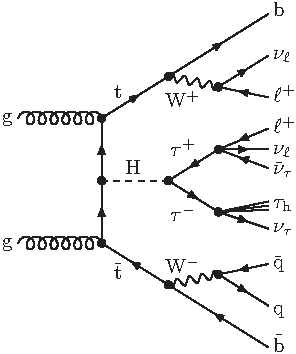
\includegraphics[width=0.30\linewidth]{diagrams/gg-ttH-tt-2lss.pdf} 
\hspace{0.5cm}
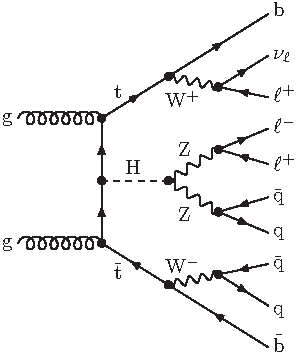
\includegraphics[width=0.30\linewidth]{diagrams/gg-ttH-ZZ-3l.pdf}
\hspace{0.5cm}
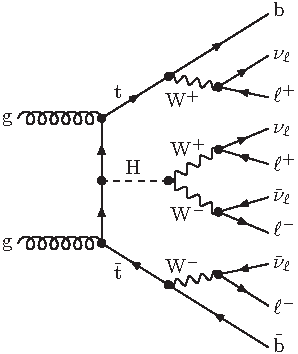
\includegraphics[width=0.30\linewidth]{diagrams/gg-ttH-WW-4l.pdf}
\caption{Examples of leading order Feynman diagrams for $t\bar{t}H$ production at pp colliders, with the Higgs boson decaying to
$\tau\tau$, $\mathrm{ZZ}^{*}$, and
$\mathrm{WW}^{*}$ (from left to right). The first, second, and third diagrams are examples of the two same-sign lepton signature,
the three lepton signature, and the four lepton signature, respectively.} 
\label{fig:feyn}
\end{figure}

\clearpage
